% Hamad Medical Corporation
% Georges Younes

\section{Geometric Algorithms for Continuous Collision Detection}\label{sec:continuous_collision}

\subsection{Collision Detection}
\label{ssec:collision_detection}
A key challenge is to develop new collision detection algorithms that can be used to check for contacts between deforming objects. One of the issues is to develop scheme that can handle topology changes that are induced by operations such as cutting and suturing. We have been working new techniques to compute the first time of contact between the models using novel continuous collision detection algorithms. Not only do they check for collisions between different objects (\eg organ and the instruments), but they also perform self-collisions between each organ. We dynamically divide the models into clusters that are guaranteed to be non-self-colliding. That way, the problem is reduced to checking for collisions between different clusters. The key issue in computing such clusters is to ensure to minimize the number of such clusters during each step of the simulation. We are currently finished the first prototype implementation and hope to test its performance on the organ benchmarks. The initial evaluation is performed on a single core \acr{cpu}, but later we would parallelize them to many-core \acr{gpu}'s. These collision algorithms would be integrated with the finite-element solvers as part of the robust surgical simulation system.

\begin{figure}
  \centering%
  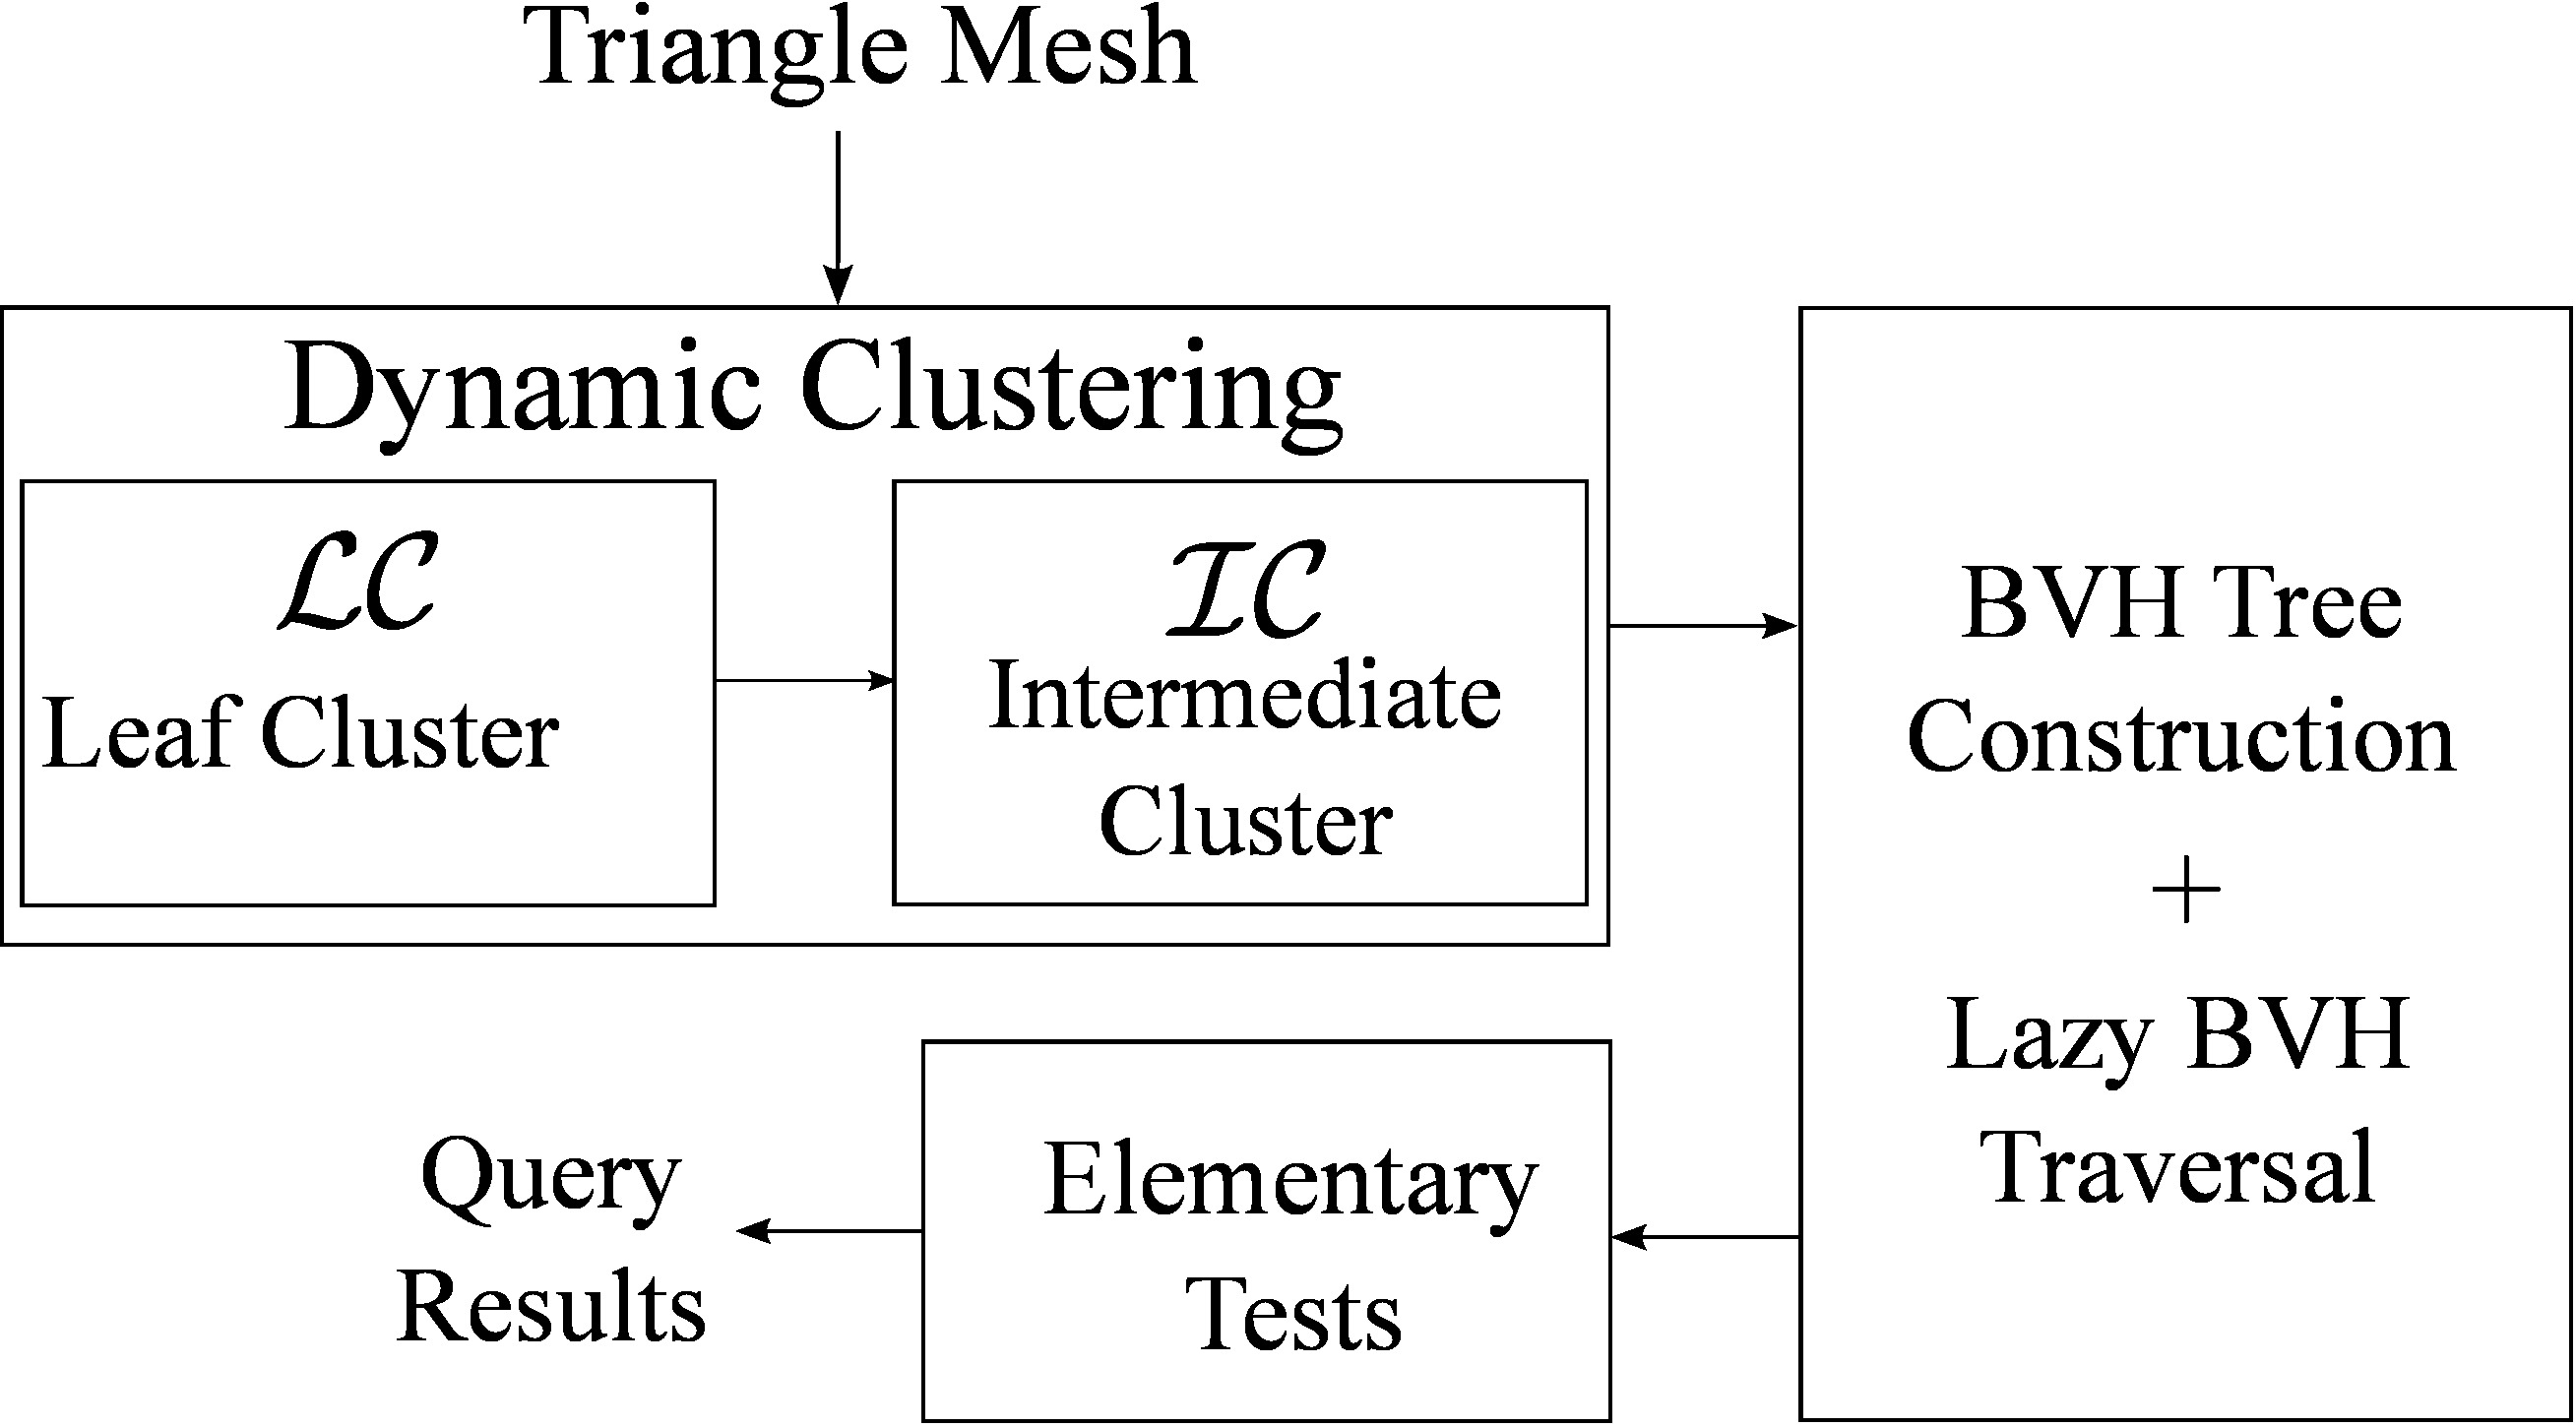
\includegraphics[width=0.55\linewidth]{collision/workflow}
  \caption{Overview of the new dynamic collision-checking algorithm that can handle models undergoing topology changes in deformable models}
  \label{fig:dynamic_collision}
\end{figure}

\subsection{Fast Continuous Collision Processing}
\label{ssec:fast_ccd}
We have  developed new algorithms for deformable collision detection using hierarchical representations. These include recomputing a new hierarchy based on the mesh topology, traversing the hierarchy and checking for overlaps, and finally between elementary tests for continuous collision detection between the triangle primitives. The continuous collision checks are performed to compute any overlaps between two discrete instances. In order to deal with the topological changes in the mesh caused by cutting operation, we keep track of the changes in mesh connectivity and the new triangles that are added or deleted between successive frames. Our work exploits the local nature of these mesh connectivity changes and performs selective update of the mesh hierarchy that is governed by these incremental changes. In order to perform the selective updates, we use a novel dynamic clustering scheme. Our clustering scheme quickly decomposes the boundary of the objects into non self-colliding clusters based on the mesh connectivity and topology information. This dynamic clustering strategy is general, efficient and involves no pre-computation and exploits the high coherence in the simulation results between successive frames of the mesh. Furthermore, we use a merging algorithm that tends to compute tighter-fitting \acr{bvh}. Such tighter hierarchy reduces the number of false positives during the traversal and ultimately reduces the number of elementary tests between the triangle primitives corresponding to the \acr{ccd} results. The cluster hierarchy is used to dynamically compute the new \acr{bvh} using a lazy approach governed by the mesh topology changes.

We assume that we are given a scene composed of one or more objects. Typically each joint organ used in the surgical simulator represents a separately object and is given as a mesh. Each object is represented as a triangle mesh and may correspond to an open or closed object. We assume that it is possible to perform a local inside/outside classification with respect to each triangle in the mesh and that each triangle normal is pointing outward. During the \acr{fem} simulation, the objects may undergo motion or deformations, which can change their topology or generate new vertices and triangles; while the connectivity information may change, we assume that the new set of objects are still represented as triangular meshes with local inside/outside classification. Given two discrete time instances in a simulation, we assume that the vertices of the objects move at a constant velocity during that time interval. If new vertices are generated due to topology changes, the \acr{ccd} problem is then posed as a problem of defining appropriate mapping between the two discrete instances. Our goal is to check whether there is any collision, including self-collisions, during that time interval, which we represent as $t \in [0, 1]$. For two triangles, this computation reduces to performing 15 elementary tests corresponding to vertex-face (VF) and edge-edge (EE) pairs. Given a \acr{ccd} query, we assume that there are no collisions among the primitives at $t = 0$. This assumption can be easily checked by using a discrete collision detection algorithm and using the simple \acr{bvh}.

The simplest general algorithms for \acr{ccd} between models undergoing topological changes (due to the cutting operation) are based on computing a \acr{bvh} of all the objects in the scene. The leaf nodes of the \acr{bvh} correspond to the triangle primitives and the intermediate nodes correspond to the bounding volumes (\eg $k$-DOP's). Prior \acr{ccd} algorithms traverse the \acr{bvh} and perform the \acr{ccd} queries between the overlapping primitives. Since the connectivity information in the mesh changes when the topology changes, prior techniques that used connectivity information to reduce the number of elementary tests are not directly applicable. As a result, prior algorithms would need to recompute the \acr{bvh} for the entire scene using top-down or bottom-up manner, which can become expensive for complex scenes with a lot of objects. In order to speed this \acr{ccd} computation, we decompose the object boundaries into dynamic clusters. Our approach uses new dynamic clustering scheme. It generates the clusters in an incremental manner by traversing the triangles on the mesh boundary, and makes no assumptions about topology or connectivity changes. We denote these clusters as leaf clusters, which correspond to the lowest level of clusters (or leaf clusters) in the final cluster hierarchy. Moreover, we ensure that each cluster has no self-collisions among its triangle primitives. As a result, \acr{ccd} reduces to querying only for inter-cluster collisions.

There are two key issues that arise in terms of computing such leaf clusters. The first issue is that, while we want to decompose the boundary into as few clusters as possible, the problem of computing that minimal number of clusters based on some standard criterion (\eg convexity) tends to be NP-hard. To overcome this issue, we compute these clusters using a greedy strategy that exploits the local connectivity and mesh changes. The second issue is that the clusters must be computed efficiently during each frame, as the object’s topology may change from frame to frame. Our next step is to merge these leaf clusters to generate the intermediate clusters; each of these intermediate clusters is also guaranteed to have no self-collisions. Our algorithm merges various neighboring leaf clusters, while the merged cluster preserve the no self-collision property. The upper level of the hierarchy are obtained by combining various intermediate clusters in a bottom-up manner. At runtime, we traverse the tree in a top down manner and check such cluster bounding volumes for collisions between them using their bounding boxes.

We have finished a preliminary implementation of this algorithm and tested its correctness on simple benchmarks. In the next six months, we propose to integrate them with the outputs of the \acr{fem} simulator that are used to implement the cutting operation.

\subsubsection{Volume Mesh}
\label{sssec:volume_mesh}
We are currently considering cutting human tissue open. When the human tissue is not cut, it is a volume and we can represent it as a watertight mesh and represent the internal materials as a discrete set of elements. When the tissue is cut, what we can do is to extend the surface mesh into the cut and stills make the mesh watertight. Our collision detection algorithm assumes that the mesh is always watertight. This assumption has been implemented using a remeshing tool.

\subsubsection{$k$-DOP}
\label{sssec:kdop}
In order to make collision detection faster, we do not directly check collision between every pair of n elements (this is $\mathrm{O}(n^2)$).  Therefore, we first use a simple geometry, \eg a box, to bound a set of fine-detailed tissues and check whether these simple geometry collides, if not we do not need costly fine-detailed collision detection checks. These fine-detailed geometry cannot be too simple, they should represent the fine-detailed tissues reasonably well, $k$-DOP's does this job better than boxes.

\subsubsection{Front Tracking}
\label{sssec:front_tracking}
Front tracking means that between timesteps, your human tissues does not change alot. So that we do not perform collision detection checks from scratch at each iteration. Instead, we keep track of what's in collision during last timestep and go from there. This makes things faster.

\subsubsection{Energy-based Collision Response}
\label{sssec:energy_based_response}
This is a method where we allow some degrees of collision to remain at every timestep, \ie we do not guarantee collisions are clearly up between timesteps. Instead, we provide a function that grows larger when you have more and deeper penetrations (collisions). Therefore, you can somewhat minimize collisions by minimizing our function.

\subsubsection{CCD vs.\ DCD}
\label{sssec:ccd_vs_dcd}
These are two modes of checking for collision detection between the geometric primitives. \acr{ccd} works in continuous time domain and checks whether the continuous movement between two timesteps will cause any  collision. If so, resolve these collisions and  until no collisions are remaining during the time interval. \acr{dcd} works in discrete time and checks whether the state of mesh at each time instance will cause collision. It does not guarantee collision-free state but runs much faster. In order to perform robust simulation, we perform \acr{ccd} computations. This also allows the underlying simulator to choose large time steps for integration.

We've included a sample screenshot of a virtual tool interacting with a virtual sphere below, and a more elaborate animated video of the interaction at \url{https://www.dropbox.com/s/8r84zjortzvh5e8/video.mp4?dl=0}.

\begin{figure}
  \centering%
	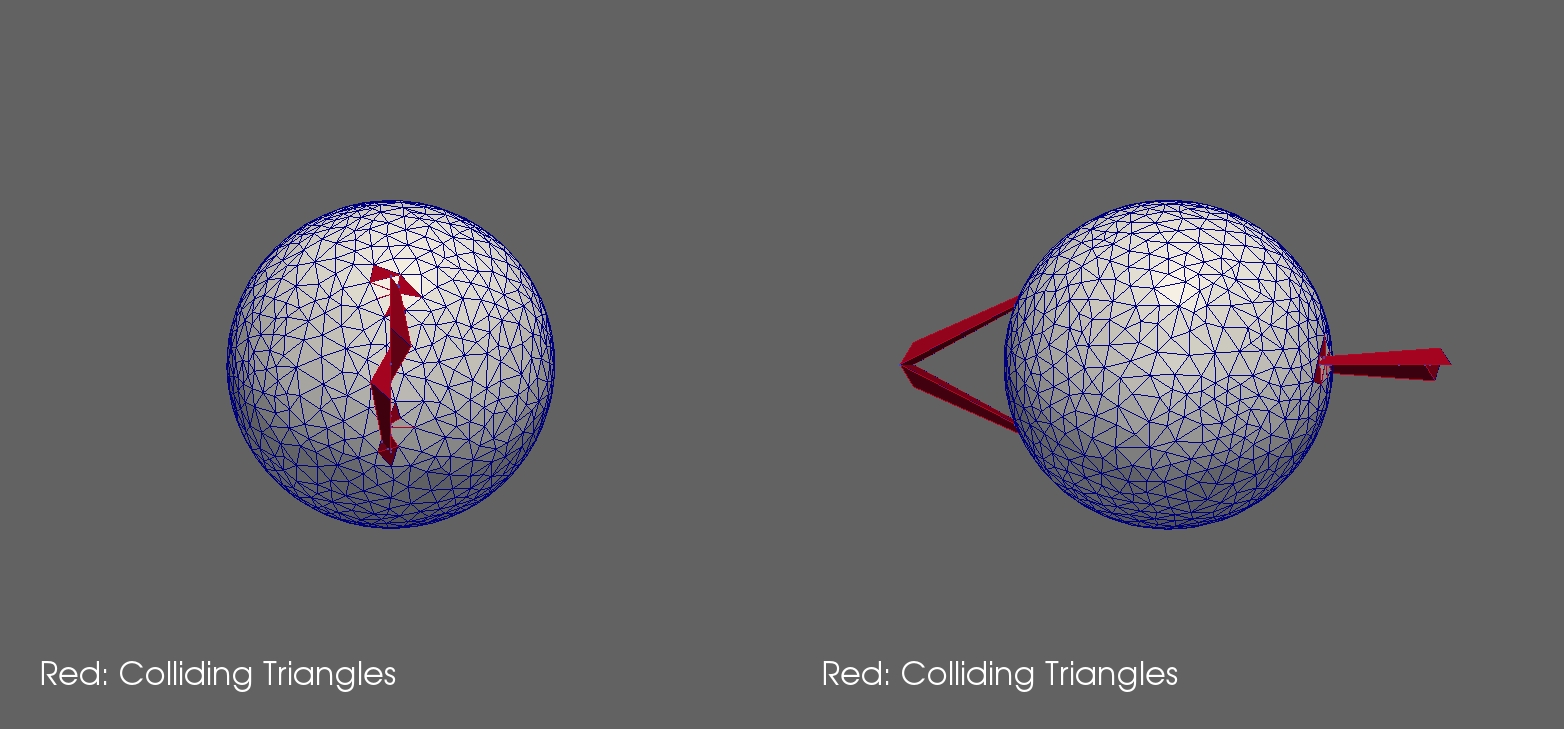
\includegraphics[width=\linewidth]{collision/cd}
	\caption{We highlight the results of our continuous collision detection between the primitives. This includes self-collision as well as collisions between the objects}
	\label{fig:cd}
\end{figure}

\subsection{Fast Collision Checking between Complex Models}
Fast collision detection and processing of the intersection of cutting tools with meshes are key operations in surgical simulation. The primary operation while cutting involves the intersection of the cutting tool trajectory with all volumetric elements of the mesh, not just the edges and faces on the boundary surfaces. As described earlier, these intersections are the starting point of the mesh subdivision operations to produce topological separation in the mesh.

The collisions involved in a cutting event must be continuous collisions where all the intersections along the path of the cutting tool movement should be reported, not just the collisions that happen at the starting and ending time instances. We first transform these continuous collisions into discrete collisions by triangulating the path of the cutting tool movement using triangle strips. After that, we detect all the edge-triangle intersections between the cutting tool path and the volumetric mesh. Note that the triangles involve both surface triangles and internal tetrahedral faces of the volumetric mesh.

Another key geometric processing operation involves the contact between the exposed boundary surface elements of the mesh and a rigid non-cutting surgical tool that can hold or push into the body but only on its exterior surface. \acr{ccd} methods are needed to robustly detect these collisions, which of course induce deformations in the volumetric mesh that are computed by the finite element model as described in Aim 2. The collisions involved in a non-cutting event can be detected following a conventional \acr{ccd} algorithm, which consists of two kinds of events: vertex-triangle intersection and edge-edge intersection.

For both cutting and non-cutting events, we use a unified \acr{bvh} to perform collision culling, which is essential for the high-performance of a collision detection system. However, most previous works only considered constructing a \acr{bvh} for a mesh with fixed topology in a precomputation step. Other methods use spatial hashing which can be used for changing topologies but involves more computation than \acr{bvh} because the spatial hashes of every element have to be updated at every frame.

To combine the merits of these two methods, we use a dynamic \acr{bvh} data structure. We construct an initial \acr{bvh} for all the surface as well as internal triangular faces for the volumetric mesh using an existing method, which minimizes the \acr{sah} cost function using a greedy algorithm. When edge or vertex intersection queries are required, we first find faces in \acr{bvh} and then index into the incident edges and vertices. The choice of only constructing one \acr{bvh} for faces reduces the computational cost to update the \acr{bvh} after the vertices move.

\begin{figure}
  \centering%
  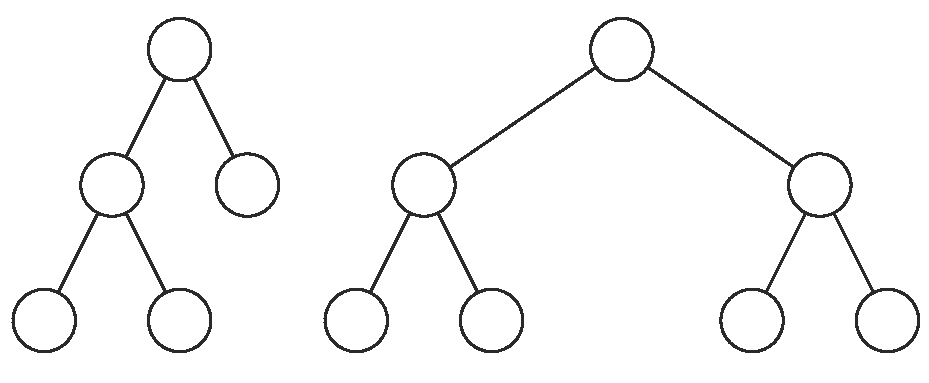
\includegraphics[width=0.8\textwidth]{collision/BVH}
  \put(-215,102){(\emph{a})}
  \put(-280,17){$C_1$}
  \put(-238,17){$C_2$}
  \put(-217,59){$C_3$}
  \put(-78,102){(\emph{b})}
  \put(-182,17){$C_1$}
  \put(-141,17){$C_2$}
  \put(-60,17){$C_3$}
  \put(-18,17){$C_4$}
  \vspace{-10px}
  \caption{An illustration of iterative \acr{bvh} updation. We update the \acr{bvh} at every timestep by first visiting every node in depth first order, so that when we visit a node for the second time, its children have correct and updated bounding volume. During the second visit of an internal node, it can either has three children (\emph{a}) or four children (\emph{b}) with the next two levels. In the case of (\emph{a}), we check whether letting $C_1,C_3$ be sibling or letting $C_2,C_3$ be sibling will improve \acr{sah} cost. If so, we apply the corresponding rotation. In the case of (\emph{b}), we check whether letting $<C_1,C_3>,<C_2,C_4>$ be sibling or letting $<C_1,C_4>,<C_2,C_3>$ be sibling will improve SAH cost. If so, we apply the corresponding rotation. In summary, there are two possible rotations to be considered in both cases}
  \label{fig:BVHRotation}
  \vspace{-5pt}
\end{figure}

When a topology change happens, the change can be boiled down to two operations: adding new triangular faces and deleting existing triangular faces. When these operations happen, we update our \acr{bvh} in a brute force manner without performing any tree balancing operations. Specifically, to add a new face, we first search in the \acr{bvh} for the existing leaf node that is closest to the face, and then use the leaf node as the sibling of the new face node. To delete a face, we use its sibling as its parent node. However, after several topology changes, the \acr{bvh} may not be balanced and reconstructing the tree from scratch can be too computationally costly for a real-time application. To meet the performance requirements, we choose to use a strategy that balances the tree in a greedy and iterative manner. After every frame of the \acr{fem} simulation, mesh vertices will move and \acr{bvh} is updated accordingly. This update will visit the entire tree and the nodes in a depth-first manner. When each non-leaf node is visited in this process, we check whether a left-rotation or a right-rotation in the AVL tree balancing algorithm will help reduce the \acr{sah}-cost. If so, the operation is applied to the node, as illustrated in \autoref{fig:BVHRotation}. Note that this modification to the \acr{bvh} update algorithm does not increase the computational complexity, and the complexity of \acr{bvh} update is still linear in the number of tree nodes. Finally \acr{gpgpu} implementations are now available, and Aim 4 is continuing integration efforts into the final prototype.

\hrule%

\subsection{Progress during the last six months}
During the past period, we have updated the collision detection module (algorithm and routines) to support various detection queries. These queries are needed at different stages of blade and human tissue interactions, which are part of surgical simulation. When the tip of the blade is moving along a prescribed trajectory, our detector performs \acr{ccd} to check for collisions between the trajectory of the tip and the mesh faces (trajectory/face detection). At the same time, we also perform continuous collision detection between the body of the blade and the mesh edges (body/edge detection). These two detection computations are used to update the topology of a mesh stored using half-edge data structure.

Besides collision detection, we have also updated the detector to support dynamic boundary volume hierarchy update after the topology of mesh has changed. This involves keeping track of each addition/deletion of edge/face/vertex in the half-edge mesh. During each modification, we update the \acr{bvh} to add/delete the corresponding node of the hierarchy and make sure that the hierarchy is of high quality and well-balanced so that further queries can be answered efficiently.

Finally, we have setup some standard test routines to make sure the detector works properly and evaluate its performance. This is performed by performing a set of standard mesh cuts and parity check between the \acr{bvh} data structure and the half-edge mesh after each cut. A sample animation video is available at \url{https://www.dropbox.com/s/6m4t7kwle8dp1kt/demo.mp4} to demonstrate this computation.

\subsection{Goals for the next six months}
We want to complete the integration of realtime \acr{ccd} and \acr{fem}. Given that this is the very first approach that integrates \acr{ccd} and \acr{fem}, we have to handle many non-trivial issues and obtain realtime performance. Our next goal is to perform detailed performance analysis and there are very few (or none) systems that have performed such tight integration. We demonstrated the overall performance in terms of:

\begin{enumerate}[\em i\em)]
  \item Evaluate its performance on complex benchmarks, and
  \item Demonstrate the benefits on realtime surgical simulation scenario.
\end{enumerate}

%Ultimately, we want to show the actual benefits to the driving application.

%\textcolor{Red}{Include content from PR 4 \path{aim_3_technical.pdf}}

\hrule%

\clearpage%
